\lab{Индукционный газовый разряд}

\aim{изучение свойств плазмы высокочастотного газового разряда
    методом зондовых характеристик.}

\equip{газоразрядная трубка с высокочастотным (ВЧ) генератором, источник
    постоянного тока, генератор звуковой частоты (ЗГ), осциллограф (ЭО),
    форвакуумный насос, вакуумметр, натекатель, вакуумный кран, делитель (Д),
    повторители--фазовращатели --- нерегулируемый~(ПФ1) и регулируемый~(ПФ2).}

Ионизацию в плазме можно получить с помощью высокочастотных (ВЧ)
электромагнитных переменных полей. Существуют различные способы введения ВЧ-поля
в разрядный объём. Один из них основан на использовании электромагнитной
индукции: через катушку-соленоид, в которую вставлена диэлектрическая
(например, стеклянная) газоразрядная камера, пропускается ток высокой частоты,
и внутри катушки индуцируется вихревое электрическое поле.
Силовые линии этого поля, а вместе с~ними и линии разрядного тока,
представляют собой окружности. Такой разряд называется \term{кольцевым},
\term{индукционным} или разрядом $H$-типа, что указывает
на определяющую роль магнитного поля. Именно такой способ возбуждения газового
разряда используется в нашей установке.

Другой способ возбуждения заключается в том, что высокочастотное напряжение
подаётся на электроды, которые могут непосредственно соприкасаться с разрядной
плазмой или быть изолированы от неё диэлектриками (стенками разрядной камеры).
Система двух электродов ведёт себя по отношению к переменному напряжению как
конденсатор, поэтому такие разряды называются \term{ёмкостными} или
разрядами $E$-типа.

Высокочастотные разряды успешно используются в технике. Индукционные разряды
применяются в безэлектродных генераторах плотной низкотемпературной плазмы
(в плазмотронах), применяемых, например, для плазмохимического производства
чистых
веществ. Разряды ёмкостного типа применяются в мощных газоразрядных лазерах.

Исследуем электрический пробой в высокочастотном поле. Начнём с исследования
движения электрона при низком давлении газа, когда столкновения с молекулами
происходят редко. Движение электрона в однородном переменном электрическом поле
описывается уравнением
\begin{equation*}
    m_e\frac{d^2x}{dt^2}=-eE_0\sin\omega t,
\end{equation*}
где $E_0$~--- амплитуда электрического поля. Интегрируя это уравнение, получим
\begin{equation*}
    v=v_0+\frac{eE_0}{\omega m_e}\cos\omega t,
\end{equation*}
где $v_0$~--- скорость электрона в момент $t=0$.

Мы видим, что скорость электрона периодически увеличивается и уменьшается, но в
среднем энергии от поля электрон не
получает. Так обстоит дело, пока вакуум достаточно высок. При увеличении
давления всё чаще происходят соударения
электронов с молекулами газа, однако медленные электроны не могут ионизировать
молекулы и соударяются с ними упруго.

Чтобы понять, как возникает пробой, исследуем, что происходит при упругом
соударении электрона с молекулами газа. Как уже отмечалось, при таких
соударениях электрон почти не теряет кинетической энергии, однако направление
его скорости претерпевает существенные изменения и может вновь совпасть с
изменившимся направлением электрического поля. В этом случае электрон при
дальнейшем движении не возвращает полю энергию, а вновь её получает. Часть
электронов может поэтому заметно ускоряться высокочастотным полем. Увеличение
энергии электрона продолжается до тех пор, пока она не станет достаточной для
ионизации газа. Затем процесс повторяется: при упругих столкновениях с
молекулами газа часть электронов
в электрическом поле ускоряется, вследствие чего происходят новые акты
ионизации. Таким образом, в газе накапливаются электроны и ионы. По мере
увеличения их концентрации возрастает роль процессов рекомбинации. В результате
действия этих двух факторов~--- ионизации и рекомбинации~---
устанавливается стационарное состояние плазмы.
Её концентрация и температура зависят от сорта газа, его давления,
а также от частоты и амплитуды высокочастотного поля.

\experiment
Схема установки представлена на рис.~\figref{Induction gas discharge}.
Заполненная газом диэлектрическая камера представляет собой цилиндрическую
стеклянную трубку (ее диаметр и длина указаны в описании), на одном из торцов
которой впаяны две молибденовые проволочки (зонды)
диаметром~$d$ и длиной~$l$, расположенные на некотором расстоянии друг от друга.
Другой конец трубки не запаян.
Он служит для откачки и для заполнения камеры газом. Трубка вставлена в катушку
индуктивности колебательного контура
ВЧ-генератора, работающего на частоте~$\sim10$~МГц. Камера откачивается
форвакуумным насосом и с помощью натекателя
заполняется воздухом до давления, указанного в описании работы в лаборатории.
Значение давления контролируется вакуумметром
(термопарным манометром).

\begin{figure}[h!]
    \centering
	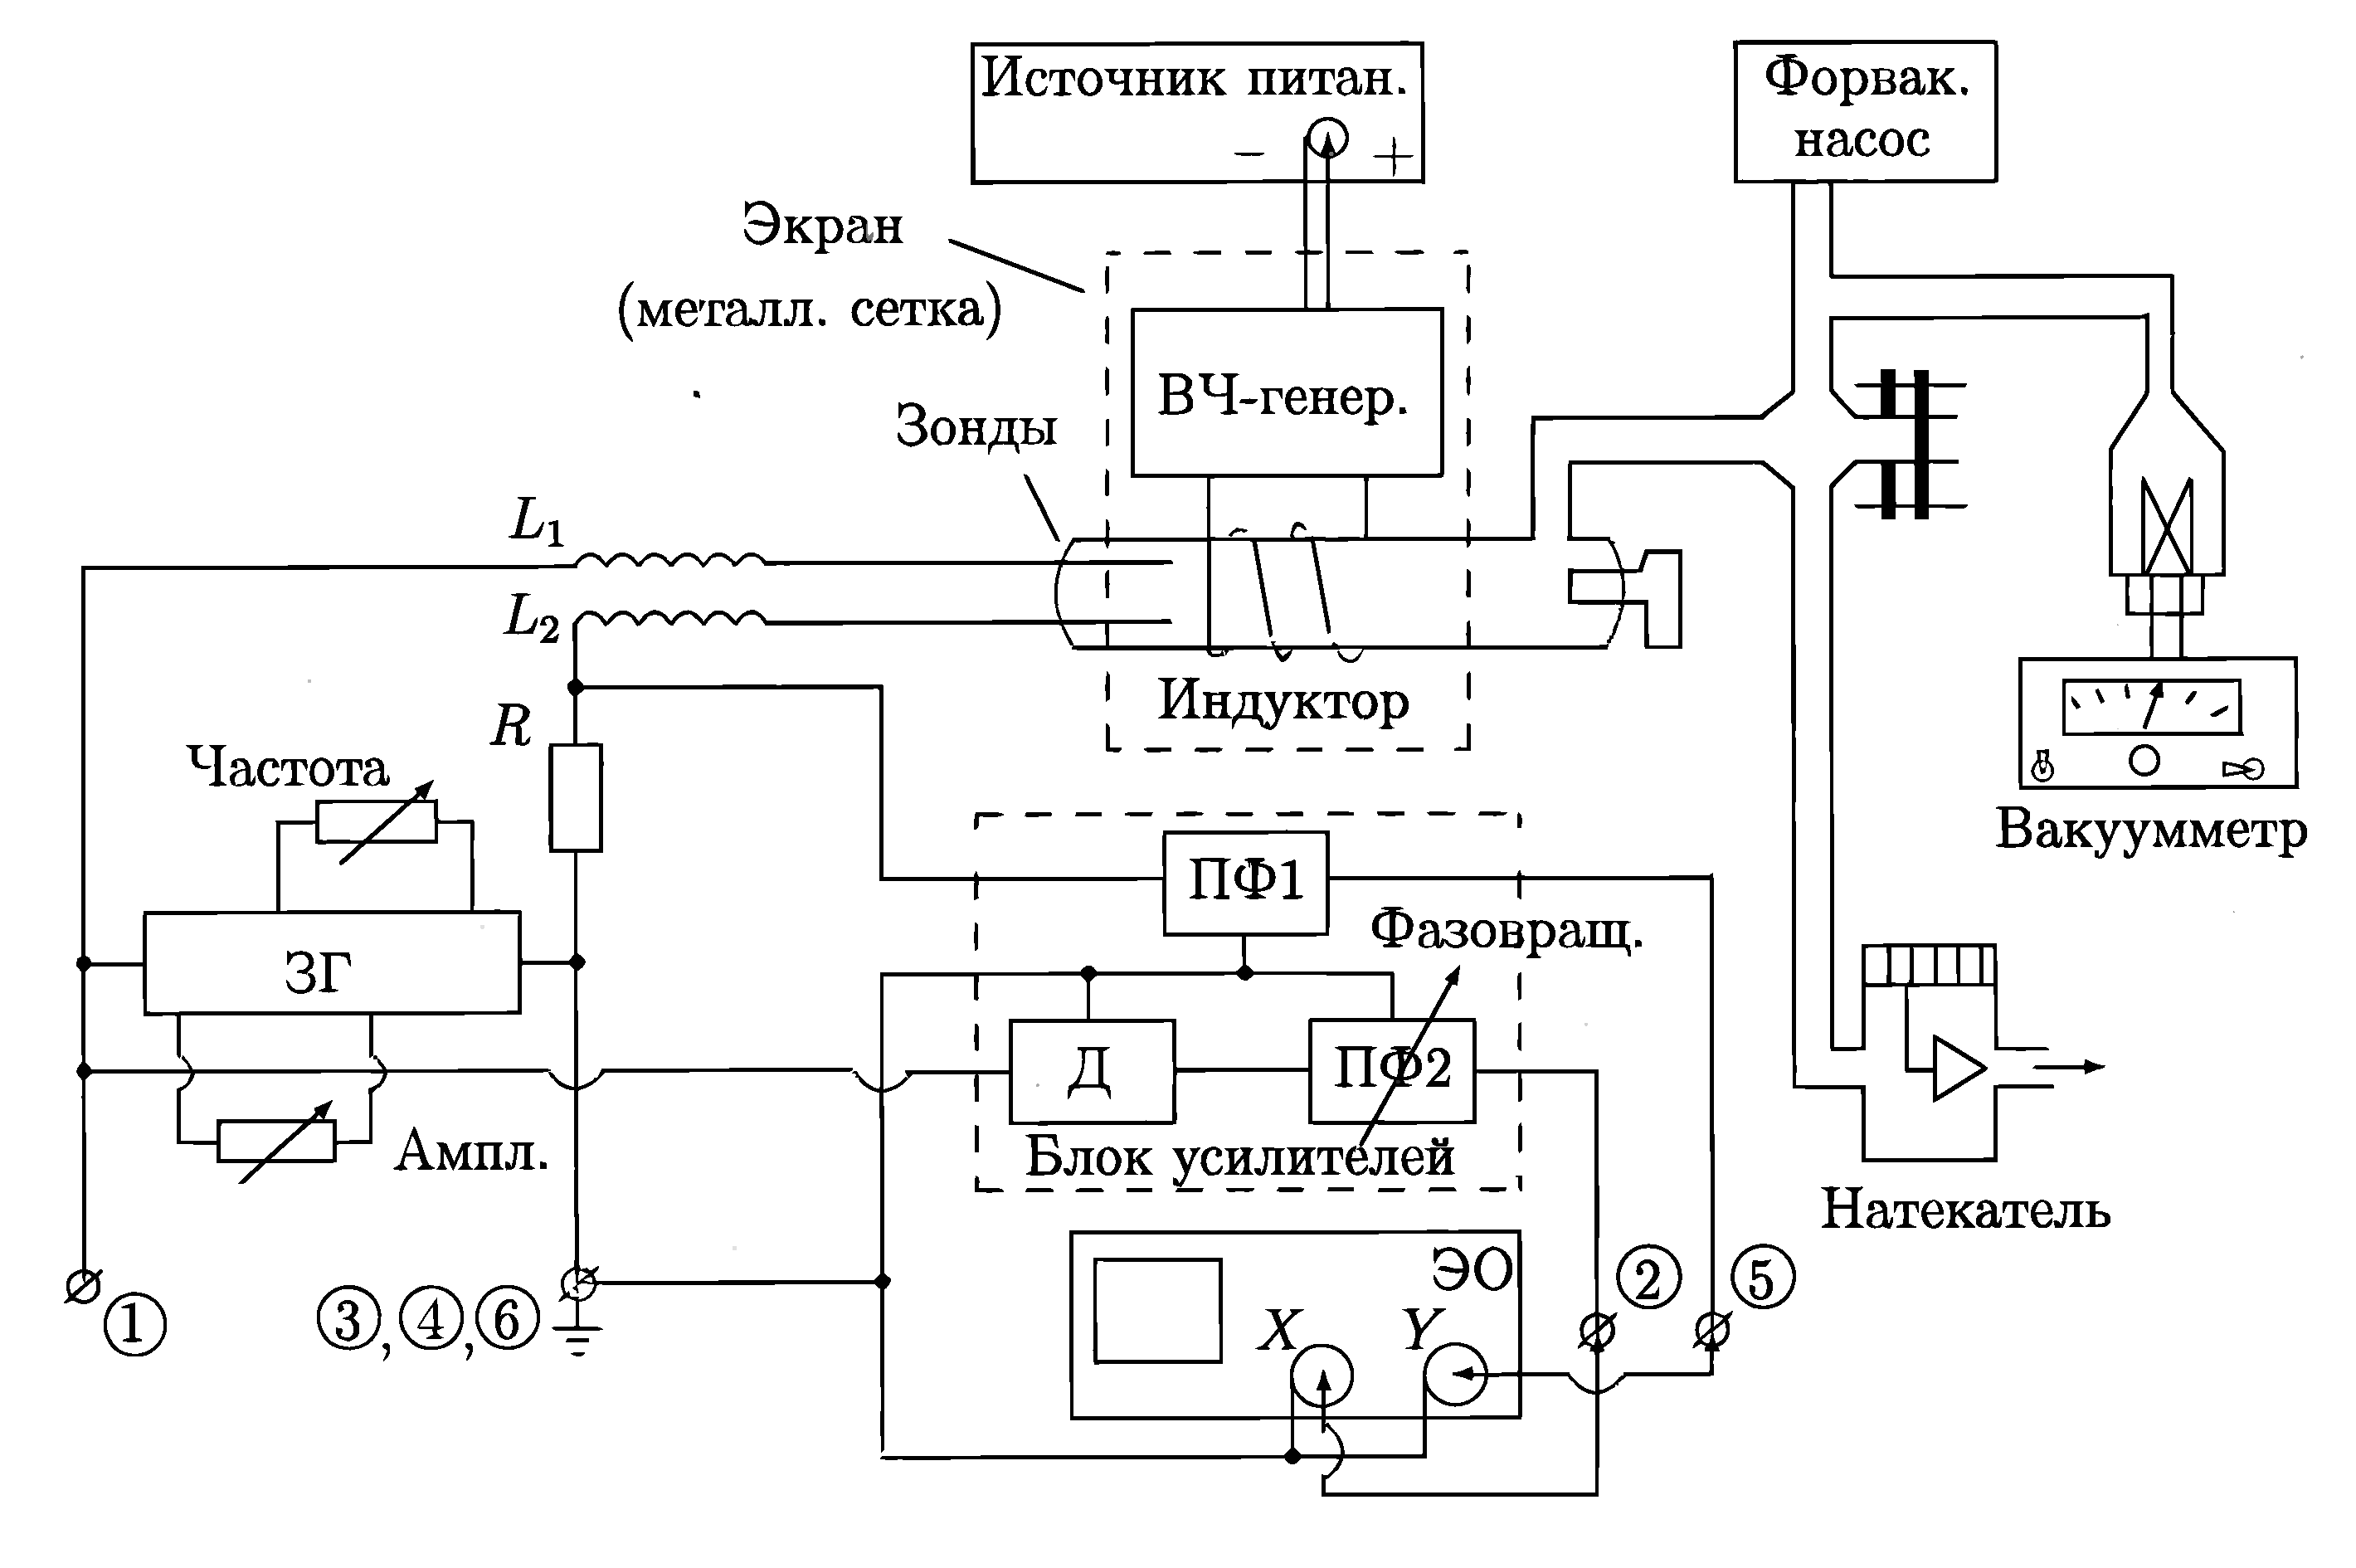
\includegraphics[width=\textwidth]{Chapter_5/3_5_2.eps}
	\caption{Схема установки для исследования газового разряда}
	\figmark{Induction gas discharge}
\end{figure}

Следует отметить некоторые особенности процедуры установки рабочего давления в
разрядной камере. Установка требуемого давления осуществляется путем изменения
проходного сечения натекателя, соединенного с атмосферой, при непрерывной работе
откачивающего насоса. При этом скорость откачки сохраняется постоянной, а приток
воздуха в разрядную камеру определяется изменением аэродинамического
сопротивления нагревателя. Таким образом, устанавливается новое значение
давления, при котором скорость откачки насоса уравновешивается расходом воздуха
через натекатель.

Изменение сечения натекателя выполняется микрометрическим винтом, который
сжимает расположенную под ним пружину и изменяет ее давление на подвижную
мембрану клапана. Такая система обладает очень большой инерциальностью и
реагирует на вращение винта со значительным запозданием.

На зонды поступает синусоидальное напряжение от звукового генератора~ЗГ.
Это же напряжение через делитель Д и регулируемый повторитель-фазовращатель ПФ2
подаётся на вход~$X$ осциллографа ЭО. Последовательно с зондом подключен датчик
тока~--- резистор~$R$ (значение сопротивления указано в описании работы).
Напряжение, пропорциональное току, текущему через плазму, подаётся на вход~$Y$
ЭО через нерегулируемый повтори-тель-фазовращатель ПФ1. Две катушки~$L_{1}$
и~$L_{2}$, подключённые к~зондам, не пропускают на осциллограф высокочастотный
сигнал.

На экране осциллографа наблюдается кривая, представляющая собой вольт-амперную
характеристику двойного зонда (см. рис.~\chapterfigref{Double probe VAC}).
Следует отметить, что на некоторых частотах в~измерительной цепи могут возникать
фазовые сдвиги, и характеристика зондов приобретает вид петли. Такие частоты
для измерений непригодны. Для устранения фазовых сдвигов используется регулятор
фазовращателя ПФ2.



\begin{lab:task}

В работе предлагается при различных давлениях газа в~трубке получить зондовые
вольт-амперные характеристики на экране
осциллографа и рассчитать с~их помощью температуру и~концентрацию электронов
в~плазме, степень ионизации, плазменную
частоту и дебаевский радиус экранирования.

\tasksection{Подготовка приборов к работе}

\begin{enumerate}
\item До включения приборов ознакомьтесь с установкой (см. описание в
лаборатории).

\item Перед откачкой ознакомьтесь с техническим описанием вакууметра,
расположенного на установке, и подготовьте его для работы. Включите форвакуумный
насос и вакуумметр. Откачайте трубку до давления, указанного в описании работы в
лаборатории. Давление
регулируется с~помощью натекателя (микровентиля) при постоянной откачке.

\item Включите источник питания ВЧ-генератора и проследите за разрядом в трубке:
после зажигания разряд должен устойчиво
гореть по всей трубке, включая область расположения зондов.


\item  Включите осциллограф и звуковой генератор, при этом на зонды подается
переменное напряжение от ЗГ с частотой, указанной в описании в лаборатории.
Подберите напряжение, при котором на экране осциллографа должна появиться
кривая, похожая на теоретическую зависимость, изображённую на
рис.~\chapterfigref{Double probe VAC}.
Если на кривой не наблюдаются области насыщения, следует увеличить выходное
напряжение~ЗГ. Если вместо кривой на экране возникает петля, ее следует изменить
регулировкой фазовращателя.

\item Посмотрите, как ведёт себя разряд, насколько он устойчив при изменении
давления в
рабочем диапазоне. Отметьте, в какой области давлений наблюдаемая на экране
кривая соответствует
теоретической.
\end{enumerate}

\tasksection{Измерения}

\begin{enumerate}
\item Получите на экране осциллографа вольт-амперную характеристику зондов
(см. рис.~\chapterfigref{Double probe VAC}) для максимального давления из
выбранного диапазона.

\item Убедитесь, что ручка плавной регулировки усиления по осям~$X$ и $Y$
выведены вправо до щелчка (при таком положении ручки чувствительность каналов
соответствует величине, указанной возле дискретного переключателя усиления).
Регулируя напряжение звукового генератора, добейтесь того, чтобы кривая
занимала почти весь экран. При чрезмерно большом напряжении генератора
возникает искажение зондовой характеристики, в ее оконечных областях появляются
изломы и выпучины. Это происходит вследствие влияния электрического поля зондов
на характер плазменного разряда. Такого допускать не следует, уменьшая
при необходимости напряжение питания зондов до исчезновения искажений.

\item Зарисуйте кривую с~экрана на кальку. Укажите на
кальке давление (в мВ и мм рт.ст.) и чувствительность осциллографа по осям $X$ и
$Y$.

\item Повторите измерения п.~6 раздела ``Подготовка приборов к работе''
для 3--4-х давлений внутри интервала, выбранного в п.~5 того же раздела.

\item Закончив работу, выключите сначала насос и немедленно откройте натекатель,
затем отключите вакууметр и остальные приборы.

\end{enumerate}

\tasksection{Обработка результатов}

\begin{enumerate}

\item Для каждой кривой пересчитайте масштаб по оси~$Y$ из В/см в А/см,
зная сопротивление, с которого сигнал, пропорциональный зондовому току,
подавался на ось~$Y$ осциллографа. Рассчитайте масштаб по оси~$X$ в~В/см
с учётом наличия делителя в канале зондового напряжения.

\item По зондовым характеристикам определите температуру~$T_e$ электронов по
формуле \chaptereqref{5.43}: ток~$I_{i\text{н}}$ найдите
из пересечения асимптоты к~току насыщения с~осью $U=0$
(см. рис.~\chapterfigref{Double probe VAC}); $(dI/dU)|_{U=0}$~--- наклон
характеристики $I(U)$ в~точке $(0,\,0)$;
определите тепловую энергию электронов~$\kB T_e$ в~электрон-вольтах.

\item Полгая концентрацию ионов и электронов одинаковой, $n_i=n_e$,
определите концентрацию электронов $n_e$ из формулы
\chaptereqref{5.43}:
\begin{equation*}
	I_{i\text{н}}=0,4n_i eS\sqrt{\frac{2kT_e}{m_i}}.
\end{equation*}
Здесь $S\approx \pi d l$~--- площадь поверхности зонда (без учёта дебаевского
слоя);
значения $d$ и $l$ приведены в описании экспериментальной установки.

\item Рассчитайте плазменную частоту колебаний электронов по формуле
\chaptereqref{plasma-freq}.
% \begin{equation}
% \omega_p=\sqrt{\frac{n_e e^2}{\varepsilon_0 m_e}}.
% \end{equation}

\item Рассчитайте дебаевский радиус экранирования~$r_{D}$ по формуле
\chaptereqref{debye-general},
которая в случае $T_{e}\gg T_{i}$ принимает вид
\begin{equation*}
    r_{D}=\sqrt{\frac{\kB T_{i}}{4\pi ne^{2}}}.
\end{equation*}
Сравните ответ с электронным дебаевским радиусом $r_{De}$
из формулы \chaptereqref{debye-rad}. Какие процессы характеризует каждая
из этих величин?

% \item Рассчитайте дебаевский радиус~$r_{D}$ экранирования по формуле
% \chaptereqref{5.18}, которая в случае $T_{e} \gg T_{i}$ принимает вид:
% \begin{equation}
% 	r_{D}=\sqrt{\frac{\varepsilon_{0}kT_{i}}{n e^{2}}}.
% \end{equation}

\item Оцените среднее число ионов в дебаевской сфере по формуле:
\begin{equation*}
    N_{D}=\frac{4\pi}{3} n_{i}r_{D}^{3}.
\end{equation*}
Является ли плазма разряда идеальной?

% \item Оцените среднее число ионов в дебаевской сфере по формуле
% \chaptereqref{5.12}.

\item Оцените степень ионизации плазмы
(долю ионизованных атомов~$\alpha$), если давление в трубке $p \simeq1$~мбар.

\item Оцените погрешности эксперимента.

\end{enumerate}

\end{lab:task}
